\section*{\textbf{1 - Normally distributed pseudo-random numbers} \hrule} 



\subsection*{\textbf{Question 1.a}}
\begin{quote}

\textbf{Problem}
\begin{quote}Write a random number generator that returns a random floating-point number between 0 and 1. At minimum, use some combination of an MWC and a 64-bit XOR-shift. Plot a sequential of random numbers against each other in a scatter plot ($x_{i+1}$ vs $x_{i}$) for the first 1000 numbers generated. Also plot the value of the random numbers for the first 1000 numbers vs the index of the random number, this mean the x-axis has a value from 0 through 999 and the y-axis 0 through 1). Finally, have your code generate 1,000,000 random numbers and plot the result of binning these in 20 bins 0.05 wide. 
\end{quote}

\textbf{Solution} 


\begin{quote}
The state of the random number generator (RNG) is updated by first performing a 64-bit XOR-shift on the current state. Next, a modified version of the 64-bit XOR-shift output is given to the MWC algorithm. The modified XOR-shifts output that is given to the MWC algorithm is the output of the 64 XOR-shift with the last 32 bits put to zero. This is done by performing the 'AND' operation with the maximum value of an unsigned int32. This modification was performed as the  MWC algorithm expects as input a 64-bit unsigned integer with a value between  $0 < x < 2^{32}$.  The output of the MWC is finally XORd with the unmodified output of the 64-bit XOR-shift. The result is set as the new state of the RNG.
\\
The first 32 bits of the new state are used to provide a random value, as the output of the MWC algorithm only contains 32 significant bits. This random value is obtained by performing the 'AND' operation between the seed and the maximum value of an unsigned int32. The resulting value is then divided by the maximum value of an unsigned int32 to obtain a value between 0 and 1.
\\
The code for the random number generator can be found at the end of this section, as it is treated as a shared module (see page \pageref{CODE:RNG}). The code for generating the plots and the created plots can be found below. The code does not only print the random seed, but also prints the maximum and minimum number of counts for the binned 1,000,000 values. These values are referred to in the description of the plot that displayed the uniformness (figure 2).
\end{quote}
\newpage

\textbf{Code - Plots}


% consists of the code that initializes the random number generator and calls the function.

\begin{quote}
The code for generating the plots. The used imports and the initialization of the random number generator are not explicit shown in this piece of code, but can be found on page \pageref{CODE:MAIN1}. The code for the random number generator can, as mentioned before, be found on page \pageref{CODE:RNG}.

\lstinputlisting[firstline=22,lastline=66]{./Code/assigment_1.py}
\end{quote}
\end{quote}

\textbf{Code - Output text } 
\begin{quote}
The text output produced by the code. The first value is the initial seed of the RNG. The second and third value are the maximum and minimum amount of counts for the histogram displaying the uniformness.
\lstinputlisting[firstline=0,lastline=3]{./Output/assigment1_out.txt}
\end{quote}
\newpage

\textbf{Code - Output plots}
\begin{quote}

\begin{figure}[!ht]
\centering
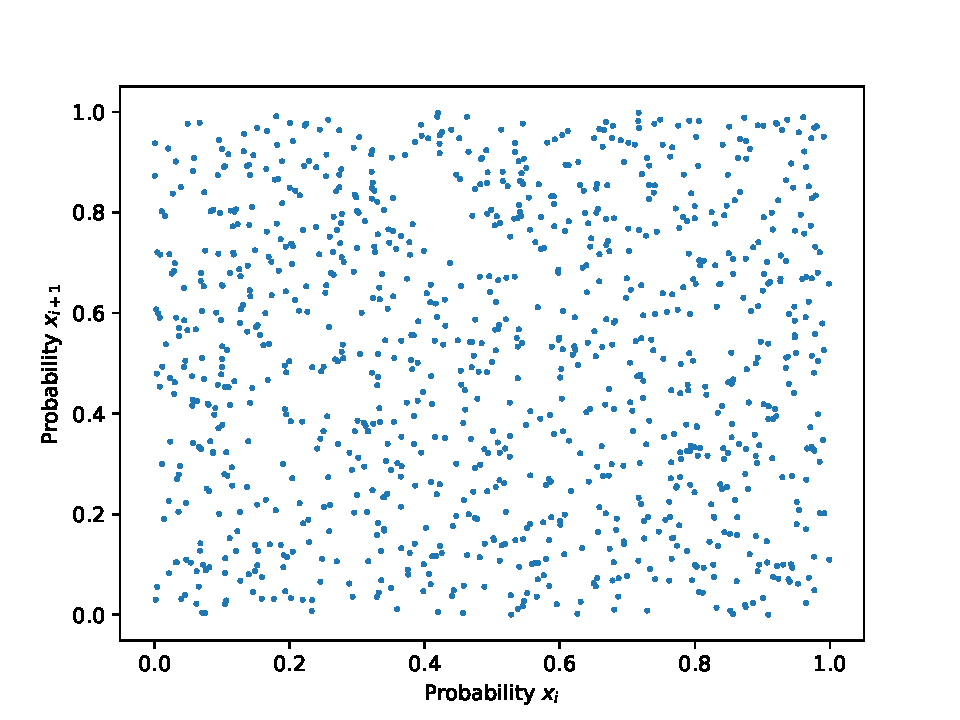
\includegraphics[width=12cm, height=7.5cm]{./Plots/1_plot_against.pdf}
\caption{A plot of random number $x_{i+1}$ against random number  $x_{i}$ for the first 1000 random uniforms produced by the random number generator. A good random number generator should produce a homogeneous plot without many (large) empty spots. The largest empty spot in the above plot is at $x_i$ = 0.4 and $x_{i+1}$ = 0.8. The spot is not significant large, but might point towards an impurity in the RNG. }
\end{figure}

\begin{figure}[!hb]
\centering
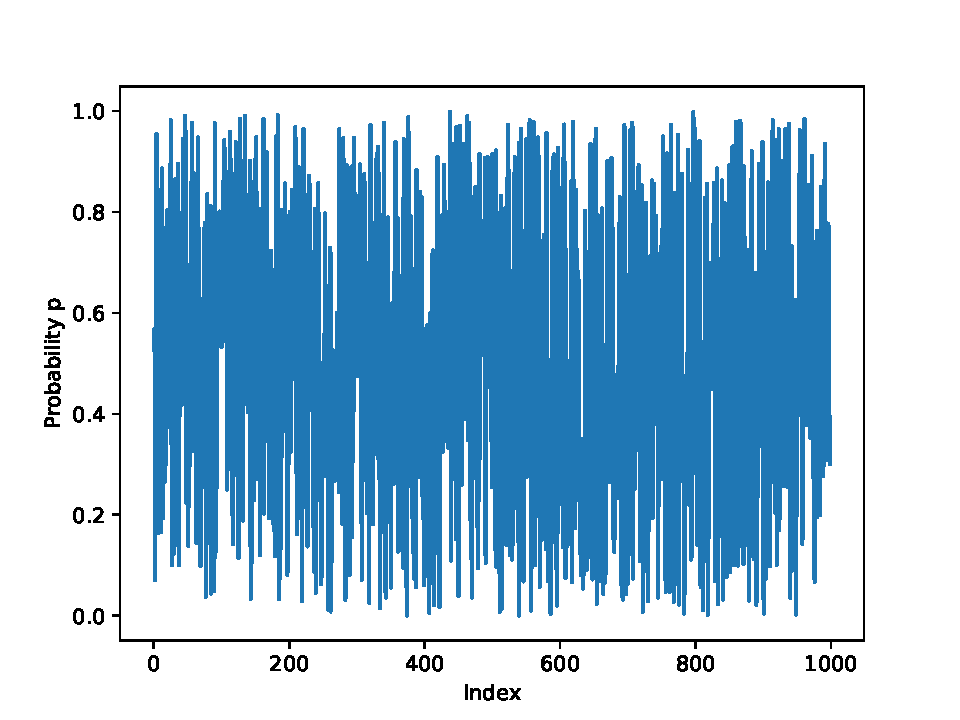
\includegraphics[width=12cm, height=8.0cm]{./Plots/1_plot_index.pdf}
\caption{The first 1000 random uniform numbers produced by the random number generator (RNG) against their index. A good random number generator should not have large wide gaps  (e.g when moving from index 400 to 450 it should not only produce values larger than 0.8, which would leave a wide gap). In the plot small gaps appear, see for example index $\sim 420$ at a probability of $ p = 0.6$. The number of gaps and the width of the gaps do not appear to be significant. This might therefore either be the result of being unlucky, or could point towards an impurity in the RNG.   The average value produced by the RNG should furthermore be 0.5. This corresponds to rapidly moving up and down around the horizontal line corresponding with a probability of $ p = 0.5$. In the plot this should, result in a 'dense' region (less white) around the line $p = 0.5$. It can indeed be seen that the plot is denser around the line $p = 0.5$ than at $ p = 0.8$ or $p = 0.2$. }
\end{figure}

\newpage
\begin{figure}[!ht]
\centering
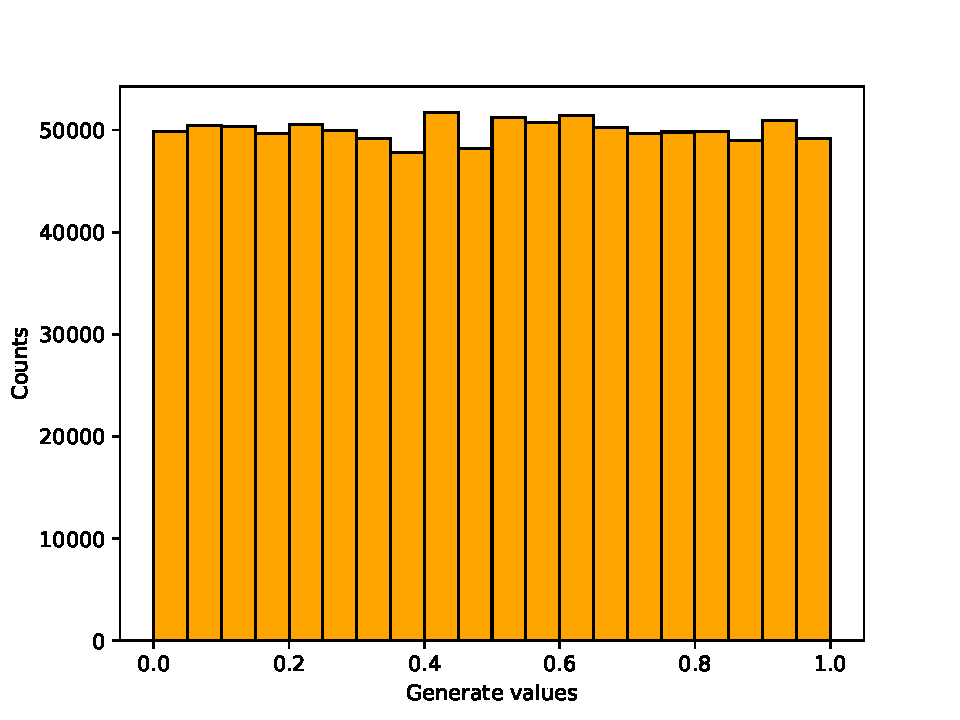
\includegraphics[width=12cm, height=7.0cm]{./Plots/1_hist_uniformnes.pdf}
\caption{The uniforms of the random number generator for 1 million random values. The values are binned in 20 bins. A good random number generator should fluctuate around 50000 $\pm 2\sqrt{50000} = 50000 \pm 447 $ counts per bin (2 sigma). The maximum and minimum amount of counts corresponds to  50343 and 49557 counts. These values just lay withing the 2 sigma uncertainty.  The uniformness of the random number generator therefore appears to be acceptable.  }
\end{figure}
\end{quote}


%\textbf{Code - helper } 
%\begin{quote}
%The code for the Poisson distribution and the factorial function.  
%\lstinputlisting[firstline=2,lastline=46]{./code/mathlib/utils.py}
%\end{quote}


%\textbf{Output}
%\begin{quote}
%The output produced by \textsf{/code/assigment1\_ a.py} 
%\lstinputlisting{./output/assigment1_a_out.txt}
%\end{quote}












